% Author: Izaak Neutelings (May 2021)
% Description: hadronic top quark jet
\usetikzlibrary{calc,math,decorations.pathreplacing}

% TikZ arrow head
\tikzset{>=latex}

% COLORS
\colorlet{myblue}{blue!70!black}
\colorlet{mydarkblue}{blue!40!black}
\colorlet{mygreen}{green!40!black}
\colorlet{myred}{red!65!black}

% Cone styles
\tikzstyle{cone}     =[thin,blue!50!black,fill=blue!50!black!30]
\tikzstyle{conebase} =[cone,fill=blue!50!black!50]

% Macro to draw a jet cone from point #2 back to #1
% #1 (optional): color
% #2: apex coordinate name
% #3: base coordinate name
% #4: full opening angle (in degrees)
% #5: eccentricity factor
\newcommand\jetcone[5][blue]{{
  \pgfmathanglebetweenpoints%
    {\pgfpointanchor{#2}{center}}%
    {\pgfpointanchor{#3}{center}}%
  \edef\ang{#4/2}       % half‑opening angle
  \edef\e{#5}           % eccentricity
  \edef\vang{\pgfmathresult} % direction of axis
  \tikzmath{%
    coordinate \conevec;
    \conevec = (#2)-(#3);
    \x    = veclen(\conevecx,\conevecy)*\e*sin(\ang)^2;
    \y    = tan(\ang)*(veclen(\conevecx,\conevecy)-\x);
    \a    = veclen(\conevecx,\conevecy)*sqrt(\e)*sin(\ang);
    \b    = veclen(\conevecx,\conevecy)*tan(\ang)*sqrt(1-\e*sin(\ang)^2);
    \angb = acos(sqrt(\e)*sin(\ang));
  }
  \coordinate (tmpL) at 
    ($(#3)-(\vang:\x pt)+(\vang+90:\y pt)$);
  % Draw full ellipse for cone base
  \draw[thin,#1!40!black,rotate=\vang,
        top color=#1!50!black!80,
        bottom color=#1!40!black!80,
        shading angle=\vang]
    (#3) ellipse({\a pt} and {\b pt});
  % Draw the “cone side” as an arc + lines back to apex
  \draw[thin,#1!40!black,rotate=\vang,rounded corners=0.001pt,
        top color=#1!90!black!20,
        bottom color=#1!50!black!50,
        shading angle=\vang]
    (tmpL) arc(180-\angb:180+\angb:{\a pt} and {\b pt})
    -- (#2) -- cycle;
}}

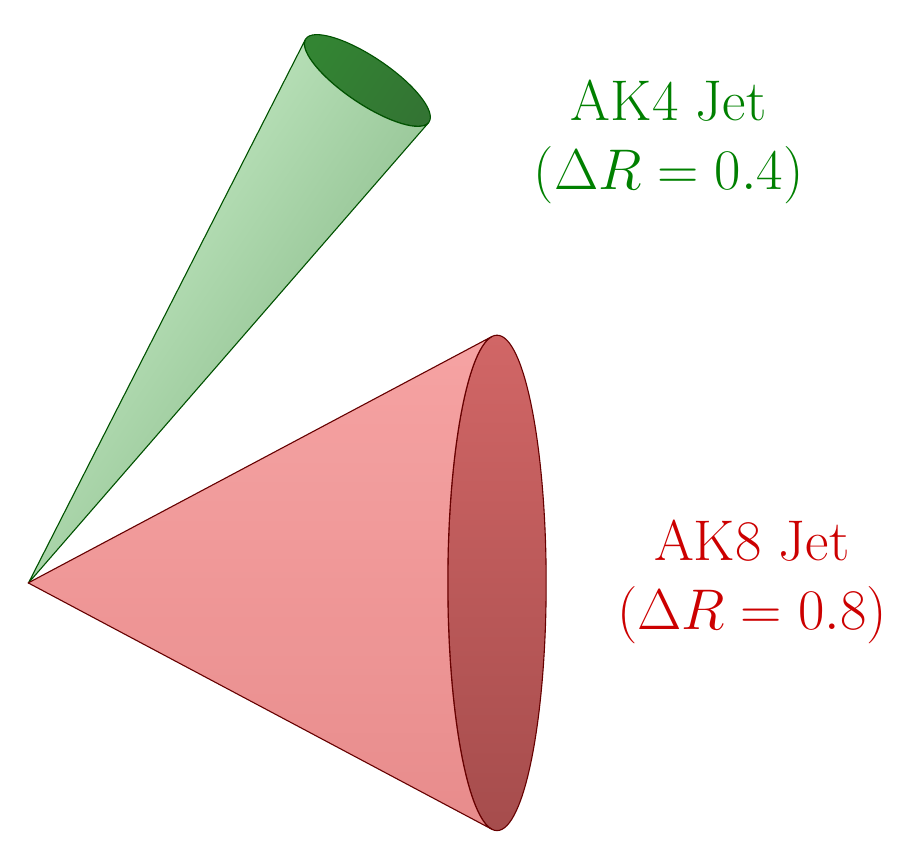
\begin{tikzpicture}[scale=7]
  % Core points
  \coordinate (O)  at (0,0);
  \coordinate (BJ) at (56:1.1);  % b‑jet axis
  \coordinate (J1) at (12:1.0);  % light q‑jet 1
  \coordinate (J2) at (-12:1.0); % light q‑jet 2
  \coordinate (M)  at (0:0.85);  % merged jet center

  % BACK of large cone
  \def\ang{28}  % full opening angle
  \def\e{0.05}  % eccentricity
  \tikzmath{%
    coordinate \axisvec;
    \axisvec = (O)-(M);
    \x    = veclen(\axisvecx,\axisvecy)*\e*sin(\ang)^2;
    \y    = tan(\ang)*(veclen(\axisvecx,\axisvecy)-\x);
    \a    = veclen(\axisvecx,\axisvecy)*sqrt(\e)*sin(\ang);
    \b    = veclen(\axisvecx,\axisvecy)*tan(\ang)*sqrt(1-\e*sin(\ang)^2);
    \angb = acos(sqrt(\e)*sin(\ang));
  }
  \coordinate (ML) at 
    ($(M)+(-180:\x pt)+(90:\y pt)$);
  % draw back half of the large cone
  \draw[thin,red!40!black,
        top color=red!70!black!60,
        bottom color=red!50!black!70]
    (M) ellipse({\a pt} and {\b pt});

  % JETS: draw three sub‑cones
  \jetcone[green!80!black]{O}{BJ}{14}{0.10} % b‑jet
  %\jetcone{O}{J1}{16}{0.08}                 % q‑jet 1
  %\jetcone{O}{J2}{16}{0.10}                 % q‑jet 2

  % Labels
  \node[green!50!black,align=center,font=\huge]
  at
    ($ (56:1.26) + (13pt,-7pt) $)
  {AK4 Jet\\$(\Delta R = 0.4)$};
  \node[red!80!black,right,align=center, font=\huge] at (0:1.05) {AK8 Jet\\$(\Delta R = 0.8)$};

  % FRONT of large cone
  \draw[thin,red!40!black,fill opacity=0.9,rounded corners=0.001pt,
        top color=red!90!black!40,
        bottom color=red!80!black!50]
    (ML) arc(180-\angb:180+\angb:{\a pt} and {\b pt})
    -- ($(O)-(0.0005,0)$) -- cycle;
\end{tikzpicture}